% Sources:
% https://github.com/koosaga/DeobureoMinkyuParty/blob/master/teamnote.tex
% https://github.com/kth-competitive-programming/kactl
% https://github.com/jacynkaa/kactl/

\begin{misc}{Pick's theorem}
	For a simple polygon with integer vertices, area $A$, $i$ grid points in the interior, and $b$ grid points on the boundary:
	$A=i+b/2-1$.
\end{misc}

\begin{misc}{Tutte matrix (perfect matching test)}
	\begin{equation*}
		M_{ij} =
			\begin{cases}
				x_{ij} & \text{if } ij \in E, i < j \\
				-x_{ji} & \text{if } ij \in E, i > j \\
				0 & \text{otherwise}
			\end{cases}
	\end{equation*}
	$\det(M) = 0 \iff $ no perfect matching w.h.p. \\
\end{misc}

\begin{misc}{Kirchhoff's theorem (\# of spanning trees)}
	\begin{equation*}
		M_{ij} =
			\begin{cases}
				\text{deg}_{\text{in}}(i) & \text{if } i = j \\
				-\#(ij\text{ edges}) & \text{if } i \neq j
			\end{cases}
	\end{equation*}
	$M' = M$ with $i$-th row and column removed \\
	$\det(M') = $ \# of oriented spanning trees rooted at $i$
\end{misc}

\begin{misc}{Cayley's formula (\# of labelled trees)}
	For degree sequence $d_1, ..., d_n$:
	\begin{equation*}
		\frac{(n-2)!}{(d_1 - 1)!(d_2 - 1)! \cdots (d_n - 1)!}
	\end{equation*}
	$n_1n_2...n_kn^{k-2} =$ for $k$ existing trees of size $n_i$ \\
	$kn^{n-k-1} =$ forests on $n$ vertices with $k$ components such that $1, ..., k$ belong to different components \\
	$x_1 \ldots x_n(x_1+ \ldots +x_n)^{n-2} = \sum_T x_1^{d_1(T)} \ldots x_n^{d_n(T)}$
\end{misc}

\begin{misc}{\# of partitions into positive integers}
	\begin{align*}
		p(0) &= 1 \\
		p(n) &= \sum_{k \in \mathbb{Z} \setminus \{0\}} (-1)^{k+1} p(n - k(3k-1)/2)
	\end{align*}
\end{misc}

\begin{misc}{Bernoulli numbers}
	EGF of Bernoulli numbers is $B(t)=\frac{t}{e^t-1}$ (FFT-able).
	$B[0,\ldots] = [1, -\frac{1}{2}, \frac{1}{6}, 0, -\frac{1}{30}, 0, \frac{1}{42}, \ldots]$ \\
	Sums of powers:
	\small
	\[ \sum_{i=1}^n n^m = \frac{1}{m+1} \sum_{k=0}^m \binom{m+1}{k} B_k \cdot (n+1)^{m+1-k} \]
	\normalsize
\end{misc}

\begin{misc}{Stirling numbers of the first kind}
	Number of permutations on $n$ items with $k$ cycles.
	\begin{align*}
		&c(n,k) = c(n-1,k-1) + (n-1) c(n-1,k) \\
		&\textstyle \sum_{k=0}^n c(n,k)x^k = x(x+1) \dots (x+n-1)
	\end{align*}
\end{misc}

\begin{misc}{Eulerian numbers}
	Number of permutations $\pi \in S_n$ in which exactly $k$ elements are greater than the previous element. $k$ $j$:s s.t. $\pi(j)>\pi(j+1)$, $k+1$ $j$:s s.t. $\pi(j)\geq j$, $k$ $j$:s s.t. $\pi(j)>j$.
	$$E(n,k) = (n-k)E(n-1,k-1) + (k+1)E(n-1,k)$$
	$$E(n,0) = E(n,n-1) = 1$$
	$$E(n,k) = \sum_{j=0}^k(-1)^j\binom{n+1}{j}(k+1-j)^n$$
\end{misc}

\begin{misc}{Stirling numbers of the second kind}
	Partitions of $n$ distinct elements into exactly $k$ groups.
	$$S(n,k) = S(n-1,k-1) + k S(n-1,k)$$
	$$S(n,1) = S(n,n) = 1$$
	$$S(n,k) = \frac{1}{k!}\sum_{j=0}^k (-1)^{k-j}\binom{k}{j}j^n$$
\end{misc}

\begin{misc}{Bell numbers}
	Total number of partitions of $n$ distinct elements. $B(n) =$
	$1, 1, 2, 5, 15, 52, 203, 877, 4140, 21147, \dots$. For $p$ prime,
	\[ B(p^m+n)\equiv mB(n)+B(n+1) \pmod{p} \]
	$$B(n) = \sum_{k=0}^n \binom{n}{k}\cdot B(k)$$
\end{misc}

\begin{misc}{Catalan numbers}
	\[ C_n=\frac{1}{n+1}\binom{2n}{n}= \binom{2n}{n}-\binom{2n}{n+1} = \frac{(2n)!}{(n+1)!n!} \]
	\[ C_0=1,\ C_{n+1} = \frac{2(2n+1)}{n+2}C_n,\ C_{n+1}=\sum C_iC_{n-i} \]
	${C_n = 1, 1, 2, 5, 14, 42, 132, 429, 1430, 4862, 16796, \dots}$
	\begin{itemize}[noitemsep,leftmargin=*]
		\item sub-diagonal monotone paths in an $n\times n$ grid.
		\item strings with $n$ pairs of parenthesis, correctly nested.
		\item binary trees with with $n+1$ leaves (0 or 2 children).
		\item ordered trees with $n+1$ vertices.
		\item ways a convex polygon with $n+2$ sides can be cut into triangles by connecting vertices with straight lines.
		\item permutations of $[n]$ with no 3-term increasing subseq.
	\end{itemize}
	Catalan convolution: find the count of balanced parentheses sequences consisting of $n+k$ pairs of parentheses where the first $k$ symbols are open brackets.
	\[ C^k=\frac{k+1}{n+k+1}\binom{2n+k}{n}\]
\end{misc}

\begin{misc}{Burnside's lemma}
	$G =$ group that acts on a set $X$ \\
	$X^g =$ set of elements fixed by $g \in G$ \\
	$X/G =$ set of orbits, i.e. equivalence classes by $G$
	$$|X/G| = \frac{1}{|G|} \sum_{g \in G} |X^g|$$
	If $f(n)$ counts ``configurations'' (of some sort) of length $n$, we can ignore rotational symmetry using $G = \mathbb Z_n$ to get
	$$g(n) = \frac 1 n \sum_{k=0}^{n-1}{f(\text{gcd}(n, k))} = \frac 1 n \sum_{k|n}{f(k)\phi(n/k)}.$$
\end{misc}

\begin{misc}{Sums}
	$$c^a + \ldots + c^b = \frac{c^{b+1} - c^a}{c-1} \text{~~~~~if } c \neq 1$$
	$$1 + \ldots + n = \frac{n(n+1)}{2}$$
	$$1^2 + \ldots + n^2 = \frac{n(2n+1)(n+1)}{6}$$
	$$1^3 + \ldots + n^3 = \frac{n^2(n+1)^2}{4}$$
	$$1^4 + \ldots + n^4 = \frac{n(n+1)(2n+1)(3n^2+3n-1)}{30}$$
\end{misc}

\begin{misc}{Series}
	$$e^x = 1+x+\frac{x^2}{2!}+\frac{x^3}{3!}+\dots,\,(|x|<\infty)$$
	$$\ln(1+x) = x-\frac{x^2}{2}+\frac{x^3}{3}-\frac{x^4}{4}+\dots,\,(x\leq1)$$
	$$\sqrt{1+x} = 1+\frac{x}{2}-\frac{x^2}{8}+\frac{2x^3}{32}-\frac{5x^4}{128}+\dots,\,(|x|\leq1)$$
	$$\sin x = x-\frac{x^3}{3!}+\frac{x^5}{5!}-\frac{x^7}{7!}+\dots,\,(|x|<\infty)$$
	$$\cos x = 1-\frac{x^2}{2!}+\frac{x^4}{4!}-\frac{x^6}{6!}+\dots,\,(|x|<\infty)$$
\end{misc}

\begin{misc}{Trigonometry}
	$$\sin(v\pm w) =\sin v\cos w\pm \cos v\sin w$$
	$$\cos(v\pm w) =\cos v\cos w\mp \sin v\sin w$$
	$$\sin v+\sin w =2\sin\dfrac{v+w}{2}\cos\dfrac{v-w}{2}$$
	$$\cos v+\cos w =2\cos\dfrac{v+w}{2}\cos\dfrac{v-w}{2}$$
	\scalebox{0.99}{\parbox{\linewidth}{
		\begin{align*}
			|\sin \frac{x}{2}| = \sqrt{\frac{1-\cos x}{2}} &&&
			|\cos \frac{x}{2}| = \sqrt{\frac{1+\cos x}{2}} \\
			\tan(v\pm w) =\dfrac{\tan v\pm\tan w}{1\mp\tan v\tan w} &&&
			|\tan \frac{x}{2}| = \sqrt{\frac{1-\cos x}{1+\cos x}}
		\end{align*}
	}}
	$$(V+W)\tan(v-w)/2{}=(V-W)\tan(v+w)/2$$
	where $V, W$ are lengths of sides opposite angles $v, w$.
	\begin{align*}
		a\cos x+b\sin x&=r\cos(x-\phi)\\
		a\sin x+b\cos x&=r\sin(x+\phi)
	\end{align*}
	where $r=\sqrt{a^2+b^2}, \phi=\operatorname{atan2}(b,a)$.
\end{misc}

\begin{misc}{Spherical coordinates}
	\vspace{-0.5cm}
	\begin{center}
		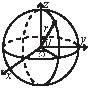
\includegraphics[width=20mm]{sphericalCoordinates}
	\end{center}
	\vspace{-0.3cm}
	\begin{align*}
		x &= r\sin\theta\cos\phi & r &= \sqrt{x^2+y^2+z^2}\\
		y &= r\sin\theta\sin\phi & \theta &= \textrm{acos}(z/\sqrt{x^2+y^2+z^2})\\
		z &= r\cos\theta & \phi &= \textrm{atan2}(y,x)
	\end{align*}
\end{misc}

\begin{misc}{Integrals}
  $$\int \sqrt{a^2+x^2} dx = \frac{x}{2}\sqrt{a^2+x^2} + \frac{a^2}{2}\ln (x+\sqrt{a^2+x^2})$$
  $$\int \sqrt{a^2-x^2} dx = \frac{x}{2}\sqrt{a^2-x^2} + \frac{a^2}{2}\arcsin\frac{x}{|a|}$$
  $$\int \frac{dx}{\sqrt{a^2-x^2}} = \arcsin\frac{x}{|a|} = -\arccos\frac{x}{|a|}$$
  $$\int \frac{dx}{\sqrt{a^2+x^2}} = \ln (x+\sqrt{a^2+x^2})$$
  $$\text{Sub } s = \tan(x/2) \text{ to get: } dx =  \frac{2\ ds}{1+s^2},$$
  $$\ \sin x = \frac{2s}{1+s^2},\ \cos x = \frac{1-s^2}{1+s^2}$$
  $$\int_a^bf(x)g(x)dx = [F(x)g(x)]_a^b-\int_a^bF(x)g'(x)dx$$
  $$\text{(Integration by parts)}$$
  $$\int\tan ax = -\dfrac{\ln|\cos ax|}{a}$$
  $$\int x\sin ax = \dfrac{\sin ax-ax \cos ax}{a^2}$$
  $$\int e^{-x^2} = \frac{\sqrt \pi}{2} \text{erf}(x), \ \ \int xe^{ax}dx = \frac{e^{ax}}{a^2}(ax-1)$$
  $$\dfrac{d}{dx}\tan x = 1+\tan^2x, \ \  \dfrac{d}{dx}\arctan x = \dfrac{1}{1+x^2}$$
  $$\text{Curve length: } \int_a^b\sqrt{1+(f'(x))^2}dx$$
  $$\text{When } X(t), Y(t): \int_a^b\sqrt{(X'(t))^2+(Y'(t))^2}dt$$
  $$\text{Solid of revolution vol: } \pi\int_a^b(f(x))^2dx$$
  $$\text{Surface area: } 2\pi\int_a^b|f(x)|\sqrt{1+(f'(x))^2}dx$$
\end{misc}

\begin{misc}{Markov chains}
	A \emph{Markov chain} is a discrete random process with the property that the next state depends only on the current state.
	Let $X_1,X_2,\ldots$ be a sequence of random variables generated by the Markov process.
	Then there is a transition matrix $\mathbf{P} = (p_{ij})$, with $p_{ij} = \Pr(X_n = i | X_{n-1} = j)$,
	and $\mathbf{p}^{(n)} = \mathbf P^n \mathbf p^{(0)}$ is the probability distribution for $X_n$ (i.e., $p^{(n)}_i = \Pr(X_n = i)$),
	where $\mathbf{p}^{(0)}$ is the initial distribution.

	$\mathbf{\pi}$ is a stationary distribution if $\mathbf{\pi} = \mathbf{\pi P}$.
	If the Markov chain is \emph{irreducible} (it is possible to get to any state from any state),
	then $\pi_i = \frac{1}{\mathbb{E}(T_i)}$ where $\mathbb{E}(T_i)$  is the expected time between two visits in state $i$.
	$\pi_j/\pi_i$ is the expected number of visits in state $j$ between two visits in state $i$.

	For a connected, undirected and non-bipartite graph, where the transition probability is uniform among all neighbors, $\pi_i$ is proportional to node $i$'s degree.

	A Markov chain is \emph{ergodic} if the asymptotic distribution is independent of the initial distribution.
	A finite Markov chain is ergodic iff it is irreducible and \emph{aperiodic} (i.e., the gcd of cycle lengths is 1).
	$\lim_{k\rightarrow\infty}\mathbf{P}^k = \mathbf{1}\pi$.

	A Markov chain is an A-chain if the states can be partitioned into two sets $\mathbf{A}$ and $\mathbf{G}$, such that all states in $\mathbf{A}$ are absorbing ($p_{ii}=1$), and all states in $\mathbf{G}$ leads to an absorbing state in $\mathbf{A}$.
	The probability for absorption in state $i\in\mathbf{A}$, when the initial state is $j$, is $a_{ij} = p_{ij}+\sum_{k\in\mathbf{G}} a_{ik}p_{kj}$.
	The expected time until absorption, when the initial state is $i$, is $t_i = 1+\sum_{k\in\mathbf{G}}p_{ki}t_k$.
\end{misc}

\begin{misc}{Pythagorean Triples}
	Uniquely generated by
	\[ a=k\cdot (m^{2}-n^{2}),\ \,b=k\cdot (2mn),\ \,c=k\cdot (m^{2}+n^{2}),\]
	$m > n > 0$, $k > 0$, $m \bot n$, and either $m$ or $n$ even.
\end{misc}

\begin{misc}{Estimates}
	The number of divisors of $n$ is at most around 100 for $n < 5e4$, 500 for $n < 1e7$, 2000 for $n < 1e10$, 200\,000 for $n < 1e19$.
\end{misc}

\begin{misc}{Mobius Function}
	\[
		\mu(n) = \begin{cases} 0 & n \textrm{ is not square free}\\ 1 & n \textrm{ has even number of prime factors}\\ -1 & n \textrm{ has odd number of prime factors}\\\end{cases}
	\]
	\[ g(n) = \sum_{d|n} f(d) \Leftrightarrow f(n) = \sum_{d|n} \mu(d)g(n/d) \]

	$ \sum_{d | n} \mu(d) = [ n = 1] $ (very useful) \\
	$ g(n) = \sum_{n|d} f(d) \Leftrightarrow f(n) = \sum_{n|d} \mu(d/n)g(d)$ \\
	$ g(n) = \sum_{1 \leq m \leq n} f(\left\lfloor\frac{n}{m}\right \rfloor ) \Leftrightarrow f(n) = \sum \mu(m)g(\left\lfloor\frac{n}{m}\right\rfloor)$
\end{misc}

\begin{misc}{Lucas' Theorem}
	Let $n,m$ be non-negative integers and $p$ a prime. Write $n=n_kp^k+...+n_1p+n_0$ and $m=m_kp^k+...+m_1p+m_0$. Then $\binom{n}{m} \equiv \prod_{i=0}^k\binom{n_i}{m_i} \pmod{p}$.
\end{misc}
